
%%%%%%%%%%%%%%%%%%%%%%%%%%%%%%%%%%%%%%%%
\documentclass{paper}
%%%%%%%%%%%%%%%%%%%%%%%%%%%%%%%%%%%%%%%%

% Declare packages in the preamble. 

% Declare some TeX packages needed for graphics. 
\usepackage{graphicx}
\usepackage{epstopdf}
\epstopdfsetup{suffix=}

% Sometimes it helps to use an if statement, 
% if you use the file on multiple platforms. 
% \ifx\pdftexversion\undefined
%     \usepackage[dvips]{graphicx}
% \else
%     \usepackage[pdftex]{graphicx}
%     \usepackage{epstopdf}
%     \epstopdfsetup{suffix=}
% \fi


%%%%%%%%%%%%%%%%%%%%%%%%%%%%%%%%%%%%%%%%
\begin{document}
%%%%%%%%%%%%%%%%%%%%%%%%%%%%%%%%%%%%%%%%

\section{Married at First Sight}

This is a document generated automatically from the figures and tables produced by
the script that was used to read in and analyze data.
First, in Section \ref{sec:data}, it describes the data.
Next, in Section \ref{sec:results}, it describes the results of the estimated regression model.

\section{Data} \label{sec:data}

Summary statistics for numerical variables are shown in Table \ref{tab:summary}.

% latex table generated in R 3.6.1 by xtable 1.8-4 package
% Sun Dec  6 13:46:24 2020
\begin{table}[ht]
\centering
\begin{tabular}{rlllllllllll}
  \hline
 &     Couple & AgeDifference & MarriedvsDivorced & DrPepperSchwartz & DrLoganLevkoff & DrJosephCilona & ChaplainGregEpstein & PastorCalvinRoberson &  RachelDeAlto & DrJessicaGriffin & DrVivianaColes \\ 
  \hline
X & Min.   : 1.00   & Min.   :0.000   & Min.   :0.0000   & Min.   :1   & Min.   :0   & Min.   :0   & Min.   :0   & Min.   :1   & Min.   :0   & Min.   :0.0   & Min.   :0.0   \\ 
  X.1 & 1st Qu.: 5.25   & 1st Qu.:0.250   & 1st Qu.:0.0000   & 1st Qu.:1   & 1st Qu.:0   & 1st Qu.:0   & 1st Qu.:0   & 1st Qu.:1   & 1st Qu.:0   & 1st Qu.:0.0   & 1st Qu.:0.0   \\ 
  X.2 & Median : 9.50   & Median :2.000   & Median :0.0000   & Median :1   & Median :0   & Median :0   & Median :0   & Median :1   & Median :0   & Median :0.5   & Median :0.5   \\ 
  X.3 & Mean   : 9.50   & Mean   :2.611   & Mean   :0.3333   & Mean   :1   & Mean   :0   & Mean   :0   & Mean   :0   & Mean   :1   & Mean   :0   & Mean   :0.5   & Mean   :0.5   \\ 
  X.4 & 3rd Qu.:13.75   & 3rd Qu.:3.750   & 3rd Qu.:1.0000   & 3rd Qu.:1   & 3rd Qu.:0   & 3rd Qu.:0   & 3rd Qu.:0   & 3rd Qu.:1   & 3rd Qu.:0   & 3rd Qu.:1.0   & 3rd Qu.:1.0   \\ 
  X.5 & Max.   :18.00   & Max.   :7.000   & Max.   :1.0000   & Max.   :1   & Max.   :0   & Max.   :0   & Max.   :0   & Max.   :1   & Max.   :0   & Max.   :1.0   & Max.   :1.0   \\ 
   \hline
\end{tabular}
\caption{Summary of Numeric Variables} 
\label{tab:summary}
\end{table}



Table \ref{tab:MarriedvsDivorced} shows the success or failure of a marriage depending on the age difference between multiple couples.

% latex table generated in R 3.6.1 by xtable 1.8-4 package
% Sun Dec  6 13:46:24 2020
\begin{table}[ht]
\centering
\begin{tabular}{rrr}
  \hline
 & Divorced & Married \\ 
  \hline
1 year age gap &   3 &   2 \\ 
  2 year age gap &   2 &   0 \\ 
  3 year age gap &   1 &   2 \\ 
  4 year age gap &   2 &   1 \\ 
  5 year age gap &   1 &   0 \\ 
  6 year age gap &   1 &   1 \\ 
  7 year age gap &   2 &   0 \\ 
   \hline
\end{tabular}
\caption{MarriedvsDivorced} 
\label{tab:MarriedvsDivorced}
\end{table}


The correlation matrix of potential variables in the model is shown in Table \ref{tab:corr}.
The success of a couple's marriage is positively correlated with the approval of Dr Pepper Schwartz and Dr Logan Levkoff. It is also can be positively correlated depending on the differences in age. In the next setion, these variables will be included in a regression model.

% latex table generated in R 4.0.2 by xtable 1.8-4 package
% Sat Dec 05 14:49:16 2020
\begin{table}[ht]
\centering
\begin{tabular}{rrrrr}
  \hline
 & AgeDifference & DrLoganLevkoff & DrPepperSchwartz & MarriedvsDivorced \\ 
  \hline
AgeDifference & 1.000 &  &  & -0.131 \\ 
  DrLoganLevkoff &  & 1.000 &  &  \\ 
  DrPepperSchwartz &  &  & 1.000 &  \\ 
  MarriedvsDivorced & -0.131 &  &  & 1.000 \\ 
   \hline
\end{tabular}
\caption{Correlation Matrix} 
\label{tab:corr}
\end{table}




\pagebreak
\section{Empirical Results}  \label{sec:results}


The estimates from the regression model are shown in Table \ref{tab:lm_model_1}.

\begin{table}
\begin{center}
\begin{tabular}{l c}
\hline
 & Model 1 \\
\hline
(Intercept)       & $2.833^{**}$ \\
                  & $(0.731)$    \\
MarriedvsDivorced & $-0.667$     \\
                  & $(1.266)$    \\
\hline
R$^2$             & $0.017$      \\
Adj. R$^2$        & $-0.044$     \\
Num. obs.         & $18$         \\
\hline
\multicolumn{2}{l}{\scriptsize{$^{***}p<0.001$; $^{**}p<0.01$; $^{*}p<0.05$}}
\end{tabular}
\caption{Regression Model 1}
\label{tab:lm_model_1}
\end{center}
\end{table}



%% Regression model description:



The regression model predicts age difference as follows 
For every approval by DrLoganLevkoff, age difference is expected 
to rise by NA. 
If the couple is approved by DrPepperSchwartz, age difference are expected 
to be NA higher. 
If there was a successful couple approved by Dr Pepper Schwartz, age difference is expected 
to be -0.667 lower. 
Overall, this model provides a fairly good description with an $R^2$ of -0.044.






\pagebreak
The regression lines are shown in Figure \ref{fig:reg}, with the estimated intercept term for marriages evaluated and approved by Dr Logan Levkoff (red), marriages evaluated and approved by both Dr Logan Levkoff and Dr Pepper Schwartz (green), and marriages evaluated and approved by Dr Logan Levkoff and rejected by Dr Pepper Schwartz.

\begin{figure}
\centering
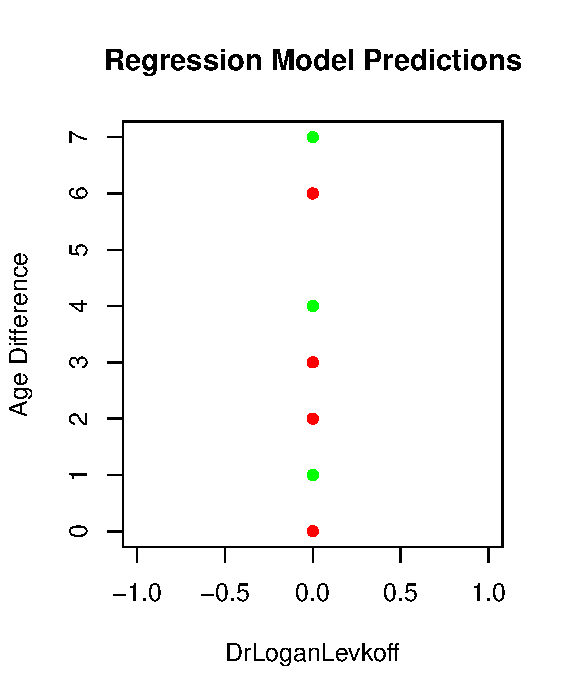
\includegraphics[width=\textwidth]{../Figures/regression.pdf}
\caption{Regression Model Predictions}
\label{fig:reg}
\end{figure}


\pagebreak
The predictions are shown in Figure \ref{fig:pred} compared to age difference.
It is clear that there is a reasonably close relationship between the predictions and the observed age differences.

\begin{figure}
\centering
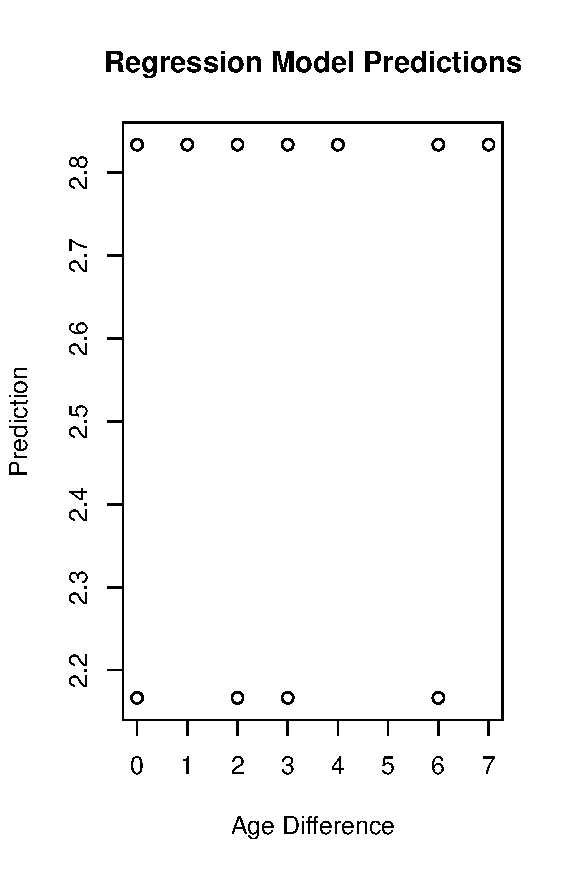
\includegraphics[width=\textwidth]{../Figures/predictions.pdf}
\caption{Age Differences vs. Predicted Age Differences}
\label{fig:pred}
\end{figure}




%%%%%%%%%%%%%%%%%%%%%%%%%%%%%%%%%%%%%%%%
\end{document}
%%%%%%%%%%%%%%%%%%%%%%%%%%%%%%%%%%%%%%%%
